\documentclass{article}

\usepackage[final]{neurips_2019}

\usepackage[utf8]{inputenc}
\usepackage[T1]{fontenc}
\usepackage{hyperref}
\usepackage{url}
\usepackage{booktabs}
\usepackage{amsmath}
\usepackage{graphicx}

\title{Cross-Species Transfer Learning with DeepSEA: From Human to Mouse}

\author{%
  Eric Xu \\
  \And
  Alexander Speltzer \\
}

\begin{document}

\maketitle

\begin{abstract}
We test whether the convolutional features a DeepSEA model learns on the human
genome transfer to mouse. We reuse the three convolutional layers of human
DeepSEA, attach a fresh multi-task head, and fine-tune on roughly one million
1000-bp windows of mouse (mm10) ENCODE data spanning 133 chromatin features.
Starting from human weights lowers validation loss faster and reaches a slightly
higher held-out AUROC (0.877) than training the same network from scratch
(0.865). The gap is small but consistent, which suggests that the early
sequence-motif detectors learned on human are partly shared across species.
\end{abstract}

\section{Introduction}

DeepSEA is a convolutional neural network that predicts chromatin features such
as transcription factor (TF) binding, DNase I hypersensitivity, and histone
marks directly from DNA sequence \citep{zhou2015deepsea}. Its first
convolutional layers act as motif detectors, learning short sequence patterns
that resemble TF binding motifs. Because the regulatory code is built from such
motifs, a natural question is whether these learned detectors are specific to the
human genome or whether they capture patterns shared across species.

We study this through transfer learning from human to mouse. If the early layers
of DeepSEA encode motifs that are conserved across species, then initializing a
mouse model with human-trained convolutional weights should help, both by
speeding up training and by improving accuracy, relative to training the same
network from random initialization. A positive result would be evidence that
DeepSEA learns common motifs rather than human-specific artifacts.

\paragraph{Related work.}
Our work builds directly on DeepSEA \citep{zhou2015deepsea}, which introduced the
architecture, the 1000-bp input window, and the multi-task formulation that
predicts hundreds of chromatin features at once. DeepSEA was trained and
evaluated only on the human genome. We keep its convolutional design and
training setup and ask whether the features it learns extend to a second species.

\section{Methods}

\paragraph{Architecture.}
We split DeepSEA into a \emph{trunk} and a \emph{head}. The trunk is the three
convolutional blocks of the original model: convolutions with 320, 480, and 960
kernels of width 8, each followed by a ReLU, with max-pooling (width 4) after the
first two blocks and dropout throughout. The trunk maps a one-hot encoded
$4 \times 1000$ input to a $960 \times L$ feature map. The head flattens this map
and applies a linear layer with a sigmoid output per feature. The head is sized
to the mouse feature set, so it is always trained from scratch. Only the trunk
can carry transferred knowledge, because the human and mouse label sets do not
line up one to one.

\paragraph{Transfer.}
Human weights come from the published DeepSEA checkpoint. The original weights
are stored as 2D convolutions with a singleton dimension, so we squeeze them to
1D convolution kernels and copy the three convolutional layers into our trunk by
shape-matched order. We then compare two conditions that share all other
settings: \textbf{Transfer}, where the trunk starts from human weights, and
\textbf{Scratch}, where the trunk starts from random initialization. As a control
we also report a \textbf{Baseline}, which uses the human trunk with an untrained
head and is evaluated with no fine-tuning.

\paragraph{Data.}
We built a DeepSEA-style multi-task dataset for mouse (mm10) from ENCODE. We
queried released narrowPeak files for TF ChIP-seq, histone ChIP-seq, and DNase-seq
across five biosamples: liver, heart, forebrain, CH12.LX, and MEL. A feature is a
(biosample, target) pair, for example \texttt{liver|CTCF}, so the same target in
several cell types counts as several features. We binned the genome into 200-bp
bins and labeled a bin positive for a feature when more than half of the bin
overlaps a peak of that feature. Each retained bin was expanded to a 1000-bp
window centered on it and one-hot encoded over $\{A, C, G, T\}$, with unknown
bases mapped to an all-zero column. We subsampled to $10^6$ windows over 133
features.

\paragraph{Training and evaluation.}
We split by chromosome to avoid leakage: chr19 is the test set and chr18 is the
validation set, both held out entirely, leaving about 945{,}000 training windows.
We train with AdamW and binary cross-entropy with logits, using a per-feature
positive weight equal to the negative-to-positive ratio (clipped to $[1, 100]$)
to handle class imbalance. We use a learning rate of $10^{-3}$ for the head,
batch size 256, a plateau learning-rate scheduler, and early stopping on
validation loss. We report per-feature AUROC and AUPRC on chr19, summarized by
their median across the 132 features that have both positive and negative labels
in the test chromosome. All models were trained on Google Colab using an NVIDIA
L4 GPU.

\section{Results}

\paragraph{Transfer trains faster and scores slightly higher.}
Table~\ref{tab:results} reports the held-out metrics for the three conditions.
The transfer model reaches a median AUROC of 0.877, just above the from-scratch
model at 0.865. The zero-shot baseline sits at chance (0.496), as expected, since
its head is never trained. Figure~\ref{fig:curves} shows that the difference in
training dynamics is clearer than the difference in final score: starting from
human weights, the validation loss drops faster and reaches its minimum of 0.7277
at epoch 5, while the from-scratch model needs until epoch 12 to reach a slightly
worse minimum of 0.7403. The human-initialized model also starts from a lower
training loss in the first epoch, indicating that the transferred filters are
already partly useful before any mouse fine-tuning.

\begin{table}[h]
  \centering
  \caption{Held-out (chr19) performance, median over 132 evaluable features.}
  \label{tab:results}
  \begin{tabular}{lcccc}
    \toprule
    Condition & Trunk init & Fine-tuned & Median AUROC & Median AUPRC \\
    \midrule
    Baseline & Human & No  & 0.496 & 0.018 \\
    Scratch  & Random & Yes & 0.865 & 0.230 \\
    Transfer & Human & Yes & \textbf{0.877} & \textbf{0.250} \\
    \bottomrule
  \end{tabular}
\end{table}

\begin{figure}[h]
  \centering
  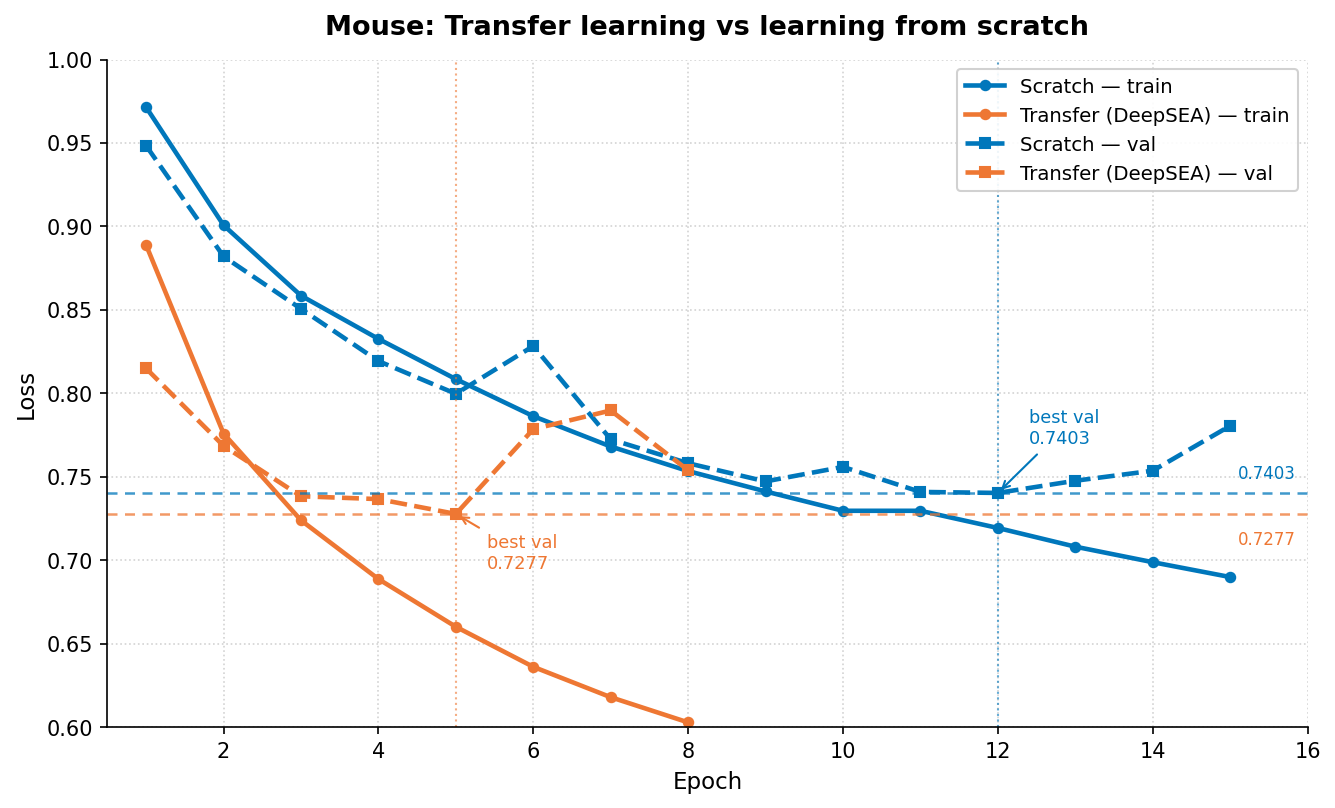
\includegraphics[width=0.75\linewidth]{figures/training_curves.png}
  \caption{Training and validation loss for transfer versus from-scratch. The
  human-initialized model (orange) decreases loss faster and reaches a lower best
  validation loss (0.7277 at epoch 5) than the random-initialized model (blue,
  0.7403 at epoch 12). Dashed horizontal lines mark each best validation loss.}
  \label{fig:curves}
\end{figure}

\paragraph{Per-feature behavior matches the original DeepSEA.}
Figure~\ref{fig:perfeature} shows the distribution of per-feature AUROC for the
transfer model. The model predicts TF and structural targets best: CTCF (across
all cell types), RAD21, SMC3, USF1/2, POLR2A, and ZC3H11A all exceed an AUROC of
0.95. The hardest features are repressive and broad histone marks such as
H3K27me3, H3K4me1, H3K36me3, and H3K79me2, which fall to 0.68 to 0.78. This
ordering, sharp TF and accessibility signals easy and broad histone marks hard,
is the same pattern reported for human DeepSEA \citep{zhou2015deepsea}.

\begin{figure}[h]
  \centering
  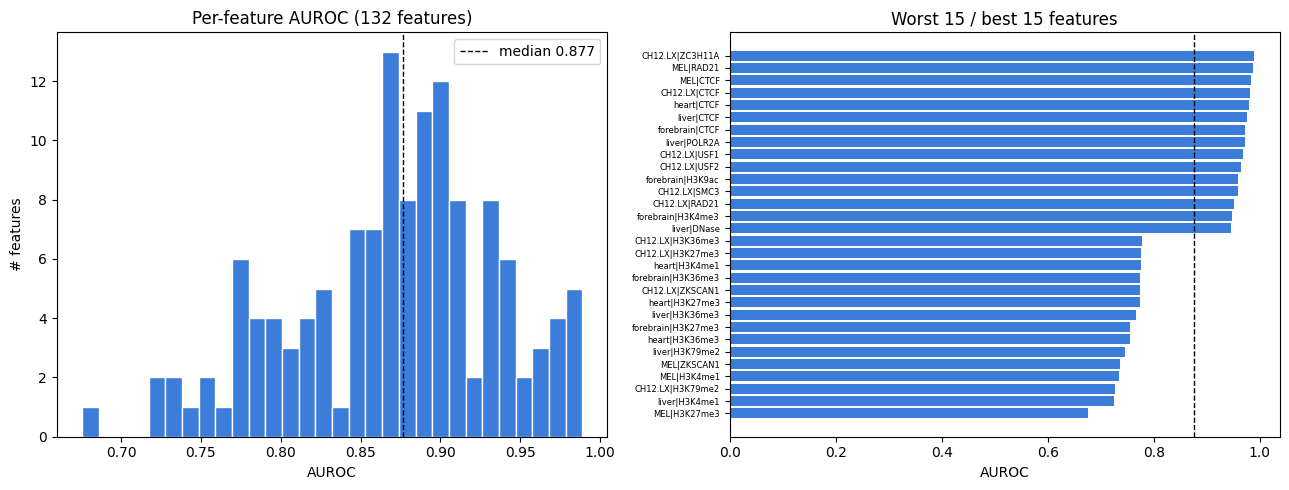
\includegraphics[width=\linewidth]{figures/transfer_learning_mouse.png}
  \caption{Per-feature AUROC of the transfer model on chr19. Left: distribution
  over 132 features, median 0.877. Right: the 15 best and 15 worst features. TF
  and structural targets (CTCF, RAD21, USF, POLR2A) score highest; broad histone
  marks score lowest.}
  \label{fig:perfeature}
\end{figure}

\section{Discussion}

Transfer learning from human to mouse works. Starting from human DeepSEA weights
lowers loss faster and gives a more accurate model than random initialization.
This supports the idea that the early convolutional layers learn motifs that are
shared between the two species, rather than features that only apply to human
sequence. We note that the accuracy gap is small, 0.877 versus 0.865 in median
AUROC, so part of it could come from run-to-run randomness. The clearer and more
reliable effect is on optimization speed, where the human-initialized model
reaches a better validation loss in fewer than half as many epochs.

\paragraph{Limitations.}
Our results are bounded by compute and by the amount of mouse data we trained on.
We capped the dataset at $10^6$ windows and stopped training early once
validation loss plateaued, so we did not push either model to its best possible
AUROC. Reaching higher accuracy would have required much longer training, which we
could not afford on a single L4 GPU. This also limits how strongly we can claim
the transfer gap is real, since a more fully trained pair of models might
converge to similar accuracy even if transfer keeps its speed advantage. Our
median AUROC of 0.877 is below the values reported for human DeepSEA, where median
AUROC was about 0.958 for TF binding, 0.923 for DNase, and 0.856 for histone
marks \citep{zhou2015deepsea}. The gap is consistent with our smaller training
budget and smaller feature set rather than a difference in the method. We leave
fuller training and the extension to more distant species for future work.

\bibliographystyle{plainnat}
\bibliography{references}

\end{document}
